%&pdflatex
\documentclass[pdftex,preprint,3p,times,numbers]{elsarticle}

\journal{Computer Physics Communications}

%\usepackage{moreverb}

\usepackage{hyperref}
\hypersetup{pdfborder={0 0 0}}

\usepackage{float}
\usepackage{wrapfig}
\usepackage{caption}
\usepackage{subcaption}
\usepackage{multirow}
\graphicspath{{images/}}

\usepackage[pdftex,usenames]{xcolor}

\usepackage{booktabs}
%\usepackage{colortbl}
\usepackage{multirow}

\usepackage{amsmath}
\usepackage{amssymb}
\usepackage[utf8x]{inputenc}
\usepackage[T1]{fontenc}

\usepackage{xspace}

\usepackage{xcolor}
\definecolor{Maroon}{cmyk}{0,0.87,0.68,0.32}
\definecolor{RoyalBlue}{cmyk}{1,0.50,0,0}
\definecolor{gray}{cmyk}{0.01,0.01,0.01,0.01}
\usepackage{listings}
\lstdefinelanguage{MyFortran}[95]{Fortran}{morecomment=[l]{\#},morestring=[d]',morekeywords={procedure,pass,deferred,non_overridable,generic,class,is}}
\lstdefinestyle{code}{%
  basicstyle=\footnotesize,%
  backgroundcolor=\color{gray},%
  language=MyFortran,%
  captionpos=b,%
  columns=fixed,%
  xleftmargin=10pt,%
  numbers=none,%
  numberstyle={\tiny},%
  keywordstyle=\color{RoyalBlue},%
  stringstyle={\sffamily},%
  texcl=true,%
  upquote=true,%
  commentstyle=\color{Maroon}%
}

\DeclareSymbolFont{extraup}{U}{zavm}{m}{n}
\DeclareMathSymbol{\vardiamond}{\mathalpha}{extraup}{87}
\definecolor{OMP}{RGB}{255,127,0}
\definecolor{MPI}{RGB}{0,127,255}
\definecolor{HYB}{RGB}{127,0,255}

\DeclareGraphicsExtensions{.pdf,.png,.jpg,.bmp,.mps}
\newcommand{\citeh}[1]{\citeauthor{#1} \citenum{#1}}

\renewcommand{\thesubfigure}{\Alph{subfigure}}

\begin{document}

\begin{frontmatter}

\title{FOODiE, Fortran Object oriented Ordinary Differential Equations integration library based on Abstract Calculus Pattern}

\author[insean]{Zaghi S.\corref{cor1}\fnref{sz}}
\ead{stefano.zaghi@cnr.it}
\fntext[sz]{Ph. D., Aerospace Engineer, Research Scientist, Dept. of Computational Hydrodynamics at CNR-INSEAN.}
\address[insean]{CNR-INSEAN, Istituto Nazionale per Studi ed Esperienze di Architettura Navale, Via di Vallerano 139, Rome, Italy, 00128}
\cortext[cor1]{Corresponding author}

\author[rsmas]{Curcic M.\fnref{mc}}
\ead{milan@orca.rsmas.miami.edu}
\fntext[mc]{Ph.D. Meteorology and Physical Oceanography, Research Scientist, Dept. of Ocean Sciences Rosenstiel School of Marine and Atmospheric Science at University of Miami}
\address[rsmas]{Ocean Sciences Rosenstiel School of Marine and Atmospheric Science, University of Miami, 4600 Rickenbacker Causeway Miami, FL 33149-1098 +1 305.421.4000}

\author[sourcery]{Rouson D.\fnref{dr}}
\ead{damian@sourceryinstitute.org}
\fntext[dr]{Ph.D. Mechanical Engineering, Founder and President Sourcery Institute and Sourcery, Inc.}
\address[sourcery]{Sourcery Institute 482 Michigan Ave., Berkeley, CA 94707}

\author[sourcery]{Beekman I.\fnref{iz}}
\ead{izaak@izaakbeekman.com}
\fntext[iz]{Graduate Research Assistant, Princeton/UMD CCROCCO LAB}

\begin{abstract}
To be written.
\end{abstract}

\begin{keyword}
  Ordinary Differential Equations (ODE) \sep
  Partial Differential Equations (PDE) \sep
  Object Oriented Programming (OOP) \sep
  Abstract Calculus Pattern (ACP) \sep
  Fortran \sep
\end{keyword}

\end{frontmatter}

{\bf PROGRAM SUMMARY}

\begin{small}
\noindent
\emph{Manuscript Title:} FOODiE, Fortran Object oriented Ordinary Differential Equations integration library based on Abstract Calculus Pattern \\
\emph{Authors:} Zaghi, S., Curcic, M., Rouson, D., Beekman, I. \\
\emph{Program title:} FOODiE \\
\emph{Journal Reference:} \\
\emph{Catalogue identifier:} \\
\emph{Licensing provisions:} GNU General Public License (GPL) v3 \\
\emph{Programming language:} Fortran (standard 2008 or newer); developed and tested with GNU gfortran 5.2 or newer \\
\emph{Computer(s) for which the program has been designed:} designed for shared-memory multi-cores workstations and for hybrid distributed/shared-memory supercomputers, but any computer system with a Fortran (2008+) compiler is suited \\
\emph{Operating system(s) for which the program has been designed:} designed for POSIX architecture and tested on GNU/Linux one \\
\emph{RAM required to execute with typical data: bytes:} $[1MB,1GB]\times core$, simulation-dependent \\
\emph{Has the code been vectorised or parallelized?:} the library is not aware of the parallel back-end, it providing a high-level models, but the provided tests suite shows parallel usage by means of MPI library and OpenMP paradigm \\
\emph{Number of processors used:} tested up to 256 \\
\emph{Supplementary material:}    \\
\emph{Keywords:} ODE, PDE, OOP, ACP, Fortran \\
\emph{CPC Library Classification:} 4.3 Differential Equations, 4.10 Interpolation, 12 Gases and Fluids \\
\emph{External routines/libraries used:} \\
\emph{CPC Program Library subprograms used:} \\
\emph{Nature of problem:} \\
Numerical integration of (general) Ordinary Differential Equations system \\
\emph{Solution method:} \\
\emph{Restrictions:} \\
\emph{Unusual features:} \\
\emph{Additional comments:} \\
\emph{Running time:} \\
\emph{References:} \\
% \begin{thebibliography}{0}
% \end{thebibliography}
\end{small}

\section{Introduction}\label{sec:introduction}
\subsection{Background}

Initial Value Problem (IVP, or Cauchy problem) constitutes a class of mathematical models of paramount relevance, it being applied to the modelling of a wide range of problems. Briefly, an IVP is an Ordinary Differential Equations system (ODE) coupled with specified initial values of the unknown state variables, the solution of which are searched at a given time after the initial time considered.

The prototype of IVP can be expressed as:
\begin{equation}
  \begin{matrix}
  U_t = R(t,U) \\
  U_0 = F(t_0)
  \end{matrix}
\label{eq:IVP}
\end{equation}
where $U(t)$ is the vector of state variables being a function of the time-like independent variable $t$, $U_t = \frac{dU}{dt} = R(t,U)$ is the (vectorial) residual function and $F$ is the (vectorial) initial conditions function evaluated at the initial time $t_0$. In general, the residual function $R$ is a function of the state variable $U$ through which it is a function of time, but it can be also a direct function of time, thus in general $R=R(t,U(t))$ holds.

The problem prototype \ref{eq:IVP} is ubiquitous in the mathematical modelling of physical problems: essentially whenever an \emph{evolutionary} phenomenon is considered the prevision (simulation) of the future solutions involves the solution of an IVP. As a matter of facts, many physical problems (fluid dynamics, chemistry, biology, evolutionary-anthropology, etc...) are described by means of an IVP.

It is worth noting that the state vector variables $U$ and its corresponding residual function $U_t = \frac{dU}{dt} = R(t,U)$ are \emph{problem dependent}: the number and the meaning of the state variables as well as the equations governing their evolution (that are embedded into the residual function) are different for the Navier-Stokes conservation laws with respect the Burgers one, as an example. Nevertheless, the \emph{solvers} used for the prediction of the Navier-Stokes equations evolution (hereafter the \emph{solution}) are the same that are used for Burgers equations time-integration. As a consequence, the solution of the IVP model prototype can be generalized, allowing the application of the same solver to many different problems, thus eliminating the necessity to re-implement the same solver for each different problem.

FOODiE library is designed for solving the generalized IVP \ref{eq:IVP}, it being completely unaware of the actual problem's definition. FOODiE library provides a high-level, well-documented, simple Application Program Interface (API) for many well-known ODE integration solvers, its aims being twofold:

\begin{itemize}
  \item provide a robust set of ODE solvers ready to be applied to a wide range of different problems;
  \item provide a simple framework for the rapid development of new ODE solvers.
\end{itemize}

{\color{red} Add citations to IVP, Cauchy, ODE references.}

\subsection{Related Works}

{\color{red} To be written.}

\subsection{Motivations and Aims}

FOODiE library must:

\begin{itemize}
  \item be written in modern Fortran (standard 2008 or newer);
  \item be written by means of Object Oriented Programming (OOP) paradigm;
  \item be well documented;
  \item be Tests Driven Developed (TDD);
  \item be collaboratively developed;
  \item be free.
\end{itemize}

FOODiE, meaning Fortran Object oriented Ordinary Differential Equations integration library, has been developed with the aim to satisfy the above specifications. The present paper is its first comprehensive presentation.

The Fortran (Formula Translator) programming language is the \emph{de facto} standard into computer science field: it strongly facilitates the effective and efficient translation of (even complex) mathematical and numerical models into an operative software without compromise on computations speed and accuracy. Moreover, its simple syntax is suitable for scientific researchers that are interested (and skilled) in the physical aspects of the numerical computations rather than computer technicians. Consequently, we develop FOODiE using Fortran language: FOODiE is written by research scientists for research scientists.

One key-point of the FOODiE development is the \emph{problem generalization}: the problem solved must be the IVP \ref{eq:IVP} rather than any of its actual definitions. Consequently, we must rely on a \emph{generic} implementation of the solvers. To this aim, OOP is very useful: it allows to express IVP \ref{eq:IVP} in a very concise and clear formulation that is really generic. In particular, our implementation is based on \emph{Abstract Calculus Pattern} (ACP) concept.

\paragraph{The Abstract Calculus Pattern}
The abstract calculus pattern provides a simple solution for the connection between the very high-level expression of IVP \ref{eq:IVP} and the eventual concrete (low-level) implementation of the ODE problem being solved. ACP essentially constitutes a \emph{contract} based on an Abstract Data Type (ADT): we specify an ADT supporting a certain set of mathematical operators (differential and integral ones) and implement FOODiE solvers only on the basis of this ADT. FOODiE clients must formulate the ODE problem under integration defining their own concrete extensions of our ADT (implementing all the deferred operators). Such an approach defines the abstract calculus pattern: FOODiE solvers are aware of only the ADT, while FOODiE clients extend the ADT for defining the concrete ODE problem.

Is is worth noting that this ACP emancipates the solvers implementations from any low-level problem-dependent details: the ODE solvers developed with this pattern are extremely concise, clear, maintainable and less errors-prone with respect a low-level (non abstract) pattern. Moreover, the FOODiE clients can use solvers being extremely robust: as a matter of facts, FOODiE solvers are expressed in a formulation very close to the mathematical one and are tested on an extremely varying family of problems. As shown in the following, such a great flexibility does not compromise the computational efficiency.

{\color{red} Add citations to Fortran standards, OOP, TDD, free software, ACP, ADT, Rouson's book references.}

\section{Mathematical and Numerical Models}\label{sec:MNmodels}

In this section the mathematical and numerical models of the currently implemented FOODiE solvers are described.

\subsection{The explicit forward Euler scheme}

{\color{red} To be written.}

\subsection{The explicit Adams-Bashforth class of schemes}

{\color{red} To be written.}

\subsection{The leapfrog solver}

{\color{red} To be written.}

\subsection{The explicit low storage Runge-Kutta class of schemes}

{\color{red} To be written.}

\subsection{The explicit TVD/SSP Runge-Kutta class of schemes}

{\color{red} To be written.}

\clearpage

\section{Application Program Interface}\label{sec:API}

In this section we review the FOODiE API providing a detailed discussion of the implementation choices.

\subsection{The main FOODiE Abstract Data Type: the integrand type}
Our ACP is based on one main ADT, the \emph{integrand} type, the definition of which is shown in listing \ref{list:type_integrand}.

\begin{lstlisting}[firstnumber=1,style=code,caption={integrand type definition},label={list:type_integrand}]
type, abstract :: integrand
  !< Abstract type for building FOODiE ODE integrators.
  contains
    ! public deferred procedures that concrete integrand-field must implement
    procedure(time_derivative),       pass(self), deferred, public:: t
    procedure(update_previous_steps), pass(self), deferred, public:: update_previous_steps
    procedure(previous_step),         pass(self), deferred, public:: previous_step
    ! operators
    procedure(symmetric_operator),   pass(lhs), deferred, public:: integrand_multiply_integrand
    procedure(integrand_op_real),    pass(lhs), deferred, public:: integrand_multiply_real
    procedure(real_op_integrand),    pass(rhs), deferred, public:: real_multiply_integrand
    procedure(symmetric_operator),   pass(lhs), deferred, public:: add
    procedure(symmetric_operator),   pass(lhs), deferred, public:: sub
    procedure(assignment_integrand), pass(lhs), deferred, public:: assign_integrand
    ! operators overloading
    generic, public:: operator(+) => add
    generic, public:: operator(-) => sub
    generic, public:: operator(*) => integrand_multiply_integrand, &
                                     real_multiply_integrand, &
                                     integrand_multiply_real
    generic, public:: assignment(=) => assign_integrand
endtype integrand
\end{lstlisting}

The \emph{integrand} type does not implement any actual integrand field, it being and abstract type. It only specifies which deferred procedures are necessary for implementing an actual concrete integrand type that can use a FOODiE solver. Listing \ref{list:type_integrand} specifies the deferred type bound procedures that clients must implement into their own concrete extension of the \emph{integrand} ADT. These procedures are analyzed in the following paragraphs.

\subsubsection{Time derivative procedure, the residual function}

The abstract interface of the time derivative procedure \emph{t} is shown in listing \ref{list:time_derivative}.

\begin{lstlisting}[firstnumber=1,style=code,caption={time derivative procedure interface},label={list:time_derivative}]
function time_derivative(self, n, t) result(dState_dt)
import :: integrand, R_P, I_P
class(integrand),       intent(IN) :: self      !< Integrand field.
integer(I_P), optional, intent(IN) :: n         !< Time level.
real(R_P),    optional, intent(IN) :: t         !< Time.
class(integrand), allocatable      :: dState_dt !< Result of the time derivative function of integrand field.
endfunction time_derivative
\end{lstlisting}

This procedure-function takes three arguments, the first passed as a \emph{type bounded} argument, while the latter are optional, and returns an integrand object. The passed dummy argument, \emph{self}, is a polymorphic argument that could be any extensions of the \emph{integrand} ADT. The optional argument \emph{n} indicated the \emph{time level} at which the residual function must be evaluated: this argument is necessary for multi-level (often referred as multi-step) solvers such as the Adams-Bashforth or leapfrog ones, but it can be omitted for other classes of solvers such the one-step multi-stages family. The optional argument \emph{t} is the {time} at which the residual function must be computed: it can be omitted in the case the residual function does not depend directly from time.

Commonly, into the concrete implementation of this deferred abstract procedure clients embed the actual ODE equations being solved. As an example, for the Burgers equation, that is a Partial Differential Equations (PDE) system involving also a boundary value problem, this procedure embeds the spatial operator that convert the PDE to a system of algebraic ODE. As a consequence, the eventual concrete implementation of this procedure can be very complex and errors-prone. Nevertheless, the FOODiE solvers are implemented only on the above abstract interface, thus emancipating the solvers implementation from any concrete complexity.

{\color{red} Add citations to Burgers, Adams-Bashfort, leapfrog references.}

\subsubsection{Update previous time steps procedure}

The abstract interface of the \emph{update previous time steps} procedure is shown in listing \ref{list:update_previous_time_steps}.

\begin{lstlisting}[firstnumber=1,style=code,caption={update previous time steps procedure interface},label={list:update_previous_time_steps}]
subroutine update_previous_steps(self, filter, weights)
import :: integrand, R_P
class(integrand),           intent(INOUT) :: self       !< Integrand field.
class(integrand), optional, intent(IN)    :: filter     !< Filter field displacement.
real(R_P),        optional, intent(IN)    :: weights(:) !< Weights for filtering the steps.
endsubroutine update_previous_steps
\end{lstlisting}

{\color{red} To be completed.}

\subsubsection{Previous step procedure}

The abstract interface of the \emph{previous step} procedure is shown in listing \ref{list:previous_step}.

\begin{lstlisting}[firstnumber=1,style=code,caption={previous step procedure interface},label={list:previous_step}]
function previous_step(self, n) result(previous)
import :: integrand, I_P
class(integrand), intent(IN)  :: self     !< Integrand field.
integer(I_P),     intent(IN)  :: n        !< Time level.
class(integrand), allocatable :: previous !< Selected previous time integrand field.
endfunction previous_step
\end{lstlisting}

{\color{red} To be completed.}

\subsubsection{Symmetric operators procedures}

The abstract interface of \emph{symmetric} procedures is shown in listing \ref{list:symmetric_operator}.

\begin{lstlisting}[firstnumber=1,style=code,caption={symmetric operator procedure interface},label={list:symmetric_operator}]
function symmetric_operator(lhs, rhs) result(operator_result)
import :: integrand
class(integrand), intent(IN)  :: lhs             !< Left hand side.
class(integrand), intent(IN)  :: rhs             !< Right hand side.
class(integrand), allocatable :: operator_result !< Operator result.
endfunction symmetric_operator
\end{lstlisting}

{\color{red} To be completed.}

\subsubsection{Integrand/real and real/integrand operators procedures}

The abstract interfaces of \emph{Integrand/real and real/integrand operators} procedures are shown in listing \ref{list:integrand_real_ops}.

\begin{lstlisting}[firstnumber=1,style=code,caption={Integrand/real and real/integrand operators procedure interfaces},label={list:integrand_real_ops}]
function integrand_op_real(lhs, rhs) result(operator_result)
import :: integrand, R_P
class(integrand), intent(IN)  :: lhs              !< Left hand side.
real(R_P),        intent(IN)  :: rhs              !< Right hand side.
class(integrand), allocatable :: operator_result  !< Operator result.
endfunction integrand_op_real

function real_op_integrand(lhs, rhs) result(operator_result)
import :: integrand, R_P
real(R_P),        intent(IN)  :: lhs             !< Left hand side.
class(integrand), intent(IN)  :: rhs             !< Right hand side.
class(integrand), allocatable :: operator_result !< Operator result.
endfunction real_op_integrand
\end{lstlisting}

{\color{red} To be completed.}

\subsubsection{Integrand assignment procedure}

The abstract interface of \emph{integrand assignment} procedure is shown in listing \ref{list:integrand_assignment}.

\begin{lstlisting}[firstnumber=1,style=code,caption={integrand assignment procedure interface},label={list:integrand_assignment}]
subroutine assignment_integrand(lhs, rhs)
import :: integrand
class(integrand), intent(INOUT) :: lhs !< Left hand side.
class(integrand), intent(IN)    :: rhs !< Right hand side.
endsubroutine assignment_integrand
\end{lstlisting}

{\color{red} To be completed.}

\clearpage

\subsection{The explicit forward Euler solver}

{\color{red} To be written.}

\subsection{The explicit Adams-Bashforth class of solvers}

{\color{red} To be written.}

\subsection{The leapfrog solver}

{\color{red} To be written.}

\subsection{The explicit low storage Runge-Kutta class of solvers}

{\color{red} To be written.}

\subsection{The explicit TVD/SSP Runge-Kutta class of solvers}

{\color{red} To be written.}

\section{Tests and Examples}\label{sec:Tests}

{\color{red} To be written.}

\clearpage

\subsection{Oscillation equations test}

{\color{red} To be completed.}

\begin{equation}
\begin{matrix}
U_t = R(U)  \\
U = \begin{bmatrix}
x \\
y
\end{bmatrix}\;\;\;
R(U) = \begin{bmatrix}
-f y \\
f x
\end{bmatrix}
\end{matrix}
\label{eq:oscillation}
\end{equation}

where the frequency is chosen as $f=10^4$. The ODE system \ref{eq:oscillation} is completed by the following initial conditions:

\begin{equation}
\begin{matrix}
  x(t_0) = 0 \\
  y(t_0) = 1
\end{matrix}
\label{eq:oscillation-ic}
\end{equation}

where $t_0=0$ is the initial time considered. The exact solution is:

\begin{equation}
\begin{matrix}
  x(t_0 + \Delta t) = X_0 cos(f \Delta t) - y_0 sin(f \Delta t) \\
  y(t_0 + \Delta t) = X_0 sin(f \Delta t) + y_0 cos(f \Delta t)
\end{matrix}
\label{eq:oscillation-exact}
\end{equation}

where $\Delta t$ is an arbitrary time step.

\subsubsection{Errors Analysis}

For the analysis of the accuracy of each solvers implemented into FOODiE library, we have integrated the Oscillation equations \ref{eq:oscillation} with different, decreasing time steps in the range $[5000, 2500, 1250, 625, 320, 100]$.

The error is estimated by the L2 norm of the difference between the exact ($U_e$) and the numerical ($U_{\Delta t}$) solutions for each time step:

\begin{equation}
  \varepsilon (\Delta t) = || U_e - U_{\Delta t} ||_2 = \sqrt{ \sum_{s=1}^{N_s} { \left(U_e(t_0 + s * \Delta t) - U_{\Delta t}(t_0 + s * \Delta t) \right)^2 }}
\label{eq:oscillation-error}
\end{equation}

Using two pairs of subsequent-decreasing time steps solution is possible to estimate the order of accuracy of the solver employed computing the \emph{observed order} of accuracy:

\begin{equation}
  p = \frac{log10 \left( \frac{\varepsilon (\Delta t_1)}{\varepsilon (\Delta t_2)} \right)}{log10 \left( \frac{\Delta t_1}{\Delta t_2} \right)}
\label{eq:oscillation-observed-order}
\end{equation}

where $\frac{\Delta t_1}{\Delta t_2}>1$.

Table \ref{tab:oscillation} summarizes the errors analysis.

\begin{table}[!ht]
  \centering
  \caption{Oscillation test errors analysis}\label{tab:oscillation}
  \resizebox{0.80\textwidth}{!}{%
  \begin{tabular}{cccccc}
    \toprule
    {\sc Solver} & {\sc Time Step} & {\sc Error X} & {\sc Error Y} & {\sc Order X} & {\sc Order Y} \\
    \cmidrule{2-6}
    \multirow{6}{*}{Adams-Bashforth 2 steps}
                 &   5000.0        &  0.109E+04    &  0.112E+04    & /             & /             \\
                 &   2500.0        &  0.246E+02    &  0.243E+02    & 5.47          & 5.53          \\
                 &   1250.0        &  0.783E+01    &  0.789E+01    & 1.65          & 1.62          \\
                 &    625.0        &  0.268E+01    &  0.272E+01    & 1.55          & 1.54          \\
                 &    320.0        &  0.976E+00    &  0.990E+00    & 1.51          & 1.51          \\
                 &    100.0        &  0.171E+00    &  0.173E+00    & 1.50          & 1.50          \\
    \cmidrule{2-6}
    \multirow{6}{*}{Adams-Bashforth 3 steps}
                 &   5000.0        &  0.816E+01    &  0.809E+01     & /            & /             \\
                 &   2500.0        &  0.266E+01    &  0.264E+01     & 1.62         & 1.62          \\
                 &   1250.0        &  0.120E+01    &  0.120E+01     & 1.15         & 1.14          \\
                 &    625.0        &  0.545E+00    &  0.543E+00     & 1.14         & 1.14          \\
                 &    320.0        &  0.223E+00    &  0.222E+00     & 1.34         & 1.34          \\
                 &    100.0        &  0.418E-01    &  0.416E-01     & 1.44         & 1.44          \\
    \cmidrule{2-6}
    \multirow{6}{*}{leapfrog 2 steps}
                 &   5000.0        &  0.151E+02    &  0.152E+02     & /            & /             \\
                 &   2500.0        &  0.500E+01    &  0.504E+01     & 1.60         & 1.59          \\
                 &   1250.0        &  0.190E+01    &  0.193E+01     & 1.40         & 1.39          \\
                 &    625.0        &  0.181E+01    &  0.181E+01     & 0.07         & 0.09          \\
                 &    320.0        &  0.157E+01    &  0.157E+01     & 0.21         & 0.21          \\
                 &    100.0        &  0.100E+01    &  0.100E+01     & 0.39         & 0.39          \\
    \cmidrule{2-6}
    \multirow{6}{*}{low storage Runge-Kutta 5 stages}
                 &   5000.0        &  0.120E+00    &  0.122E+00     & /            & /             \\
                 &   2500.0        &  0.106E-01    &  0.107E-01     & 3.51         & 3.51          \\
                 &   1250.0        &  0.935E-03    &  0.947E-03     & 3.50         & 3.50          \\
                 &    625.0        &  0.826E-04    &  0.836E-04     & 3.50         & 3.50          \\
                 &    320.0        &  0.793E-05    &  0.803E-05     & 3.50         & 3.50          \\
                 &    100.0        &  0.135E-06    &  0.137E-06     & 3.50         & 3.50          \\
    \cmidrule{2-6}
    \multirow{6}{*}{TVD/SSP Runge-Kutta 2 stages}
                 &   5000.0        &  0.316E+02    &  0.319E+02     & /            & /             \\
                 &   2500.0        &  0.892E+01    &  0.894E+01     & 1.83         & 1.84          \\
                 &   1250.0        &  0.301E+01    &  0.305E+01     & 1.57         & 1.55          \\
                 &    625.0        &  0.106E+01    &  0.107E+01     & 1.51         & 1.51          \\
                 &    320.0        &  0.387E+00    &  0.392E+00     & 1.50         & 1.50          \\
                 &    100.0        &  0.676E-01    &  0.685E-01     & 1.50         & 1.50          \\
    \cmidrule{2-6}
    \multirow{6}{*}{TVD/SSP Runge-Kutta 3 stages}
                 &   5000.0        &  0.255E+01    &  0.252E+01     & /            & /             \\
                 &   2500.0        &  0.523E+00    &  0.516E+00     & 2.28         & 2.29          \\
                 &   1250.0        &  0.944E-01    &  0.931E-01     & 2.47         & 2.47          \\
                 &    625.0        &  0.167E-01    &  0.165E-01     & 2.50         & 2.50          \\
                 &    320.0        &  0.314E-02    &  0.310E-02     & 2.50         & 2.50          \\
                 &    100.0        &  0.171E-03    &  0.169E-03     & 2.50         & 2.50          \\
    \cmidrule{2-6}
    \multirow{6}{*}{TVD/SSP Runge-Kutta 5 stages}
                 &   5000.0        &  0.139E+00    &  0.141E+00     & /            & /             \\
                 &   2500.0        &  0.122E-01    &  0.124E-01     & 3.50         & 3.50          \\
                 &   1250.0        &  0.108E-02    &  0.110E-02     & 3.50         & 3.50          \\
                 &    625.0        &  0.956E-04    &  0.969E-04     & 3.50         & 3.50          \\
                 &    320.0        &  0.937E-05    &  0.949E-05     & 3.47         & 3.47          \\
                 &    100.0        &  0.512E-06    &  0.519E-06     & 2.50         & 2.50          \\
    \bottomrule
  \end{tabular}}
\end{table}

\paragraph{Adams-Bashforth}

\begin{figure}[!ht]
  \centering
  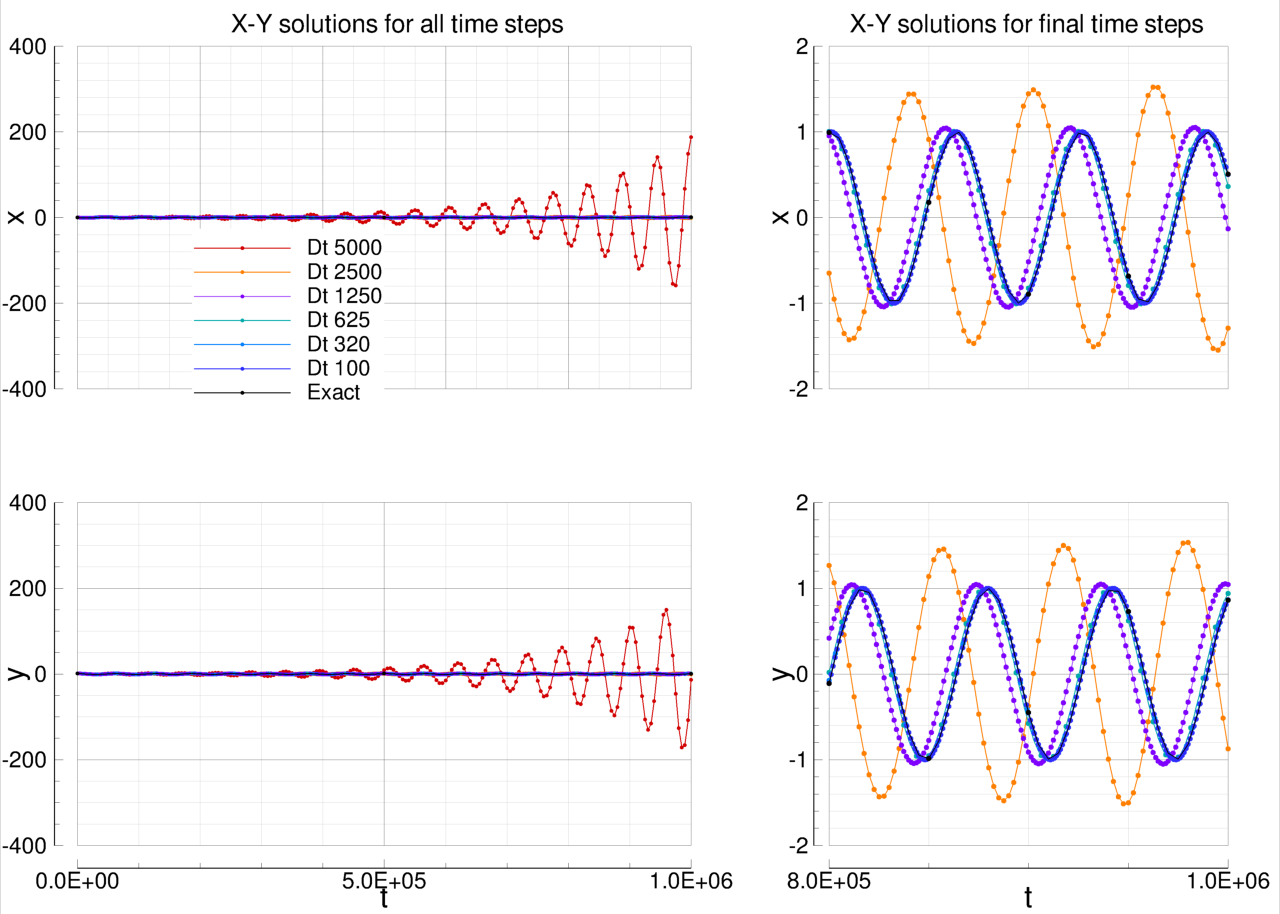
\includegraphics[width=0.70\textwidth]{errors-analysis/oscillation/errors_analysis-oscillation-adams-bashforth-2.png}
  \caption{Oscillation equations solutions computed by means of Adams-Bashforth 2 steps solver}\label{fig:results-oscillation-adams-bashforth-2}
\end{figure}

\begin{figure}[!ht]
  \centering
  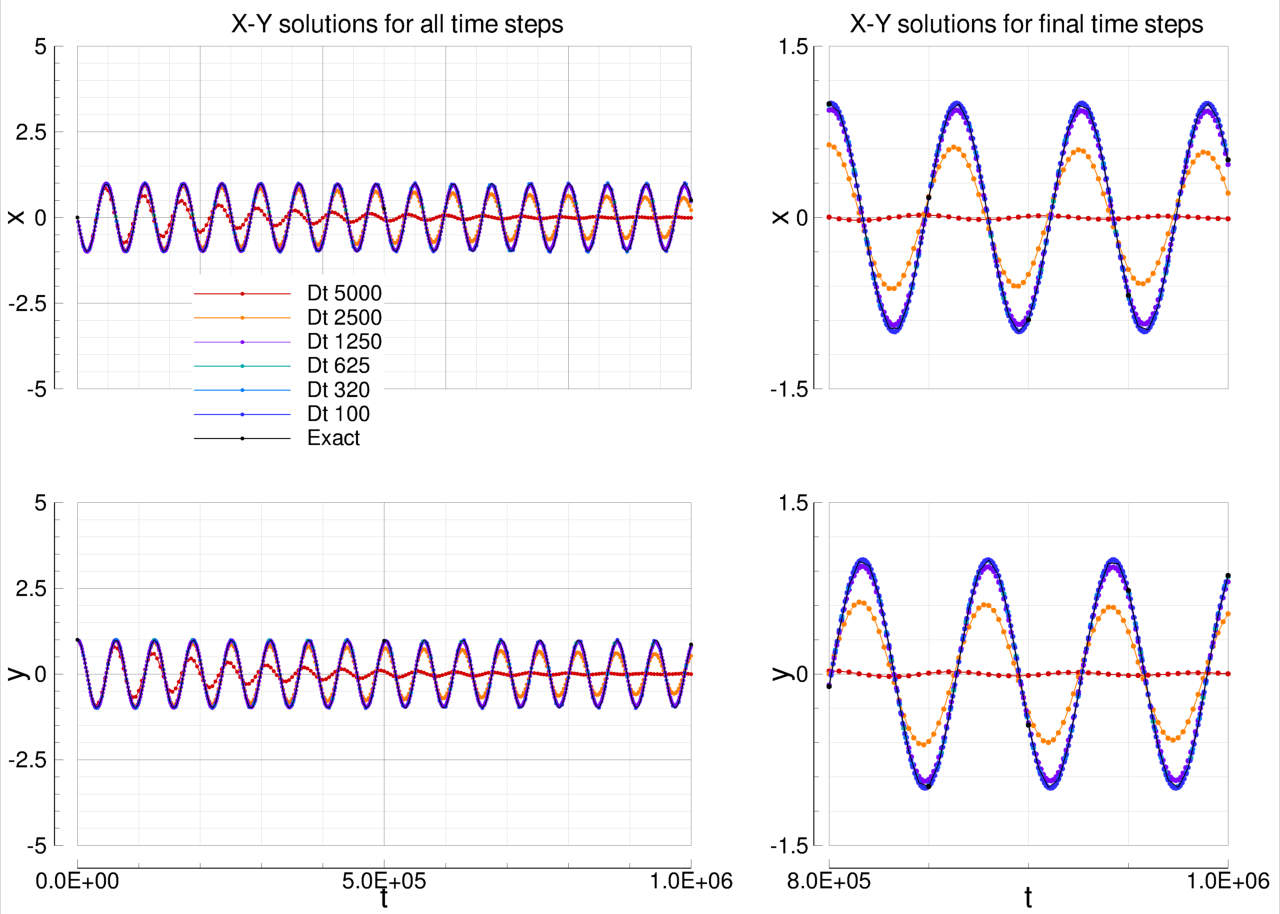
\includegraphics[width=0.70\textwidth]{errors-analysis/oscillation/errors_analysis-oscillation-adams-bashforth-3.png}
  \caption{Oscillation equations solutions computed by means of Adams-Bashforth 3 steps solver}\label{fig:results-oscillation-adams-bashforth-3}
\end{figure}

\paragraph{Leapfrog}

\begin{figure}[!ht]
  \centering
  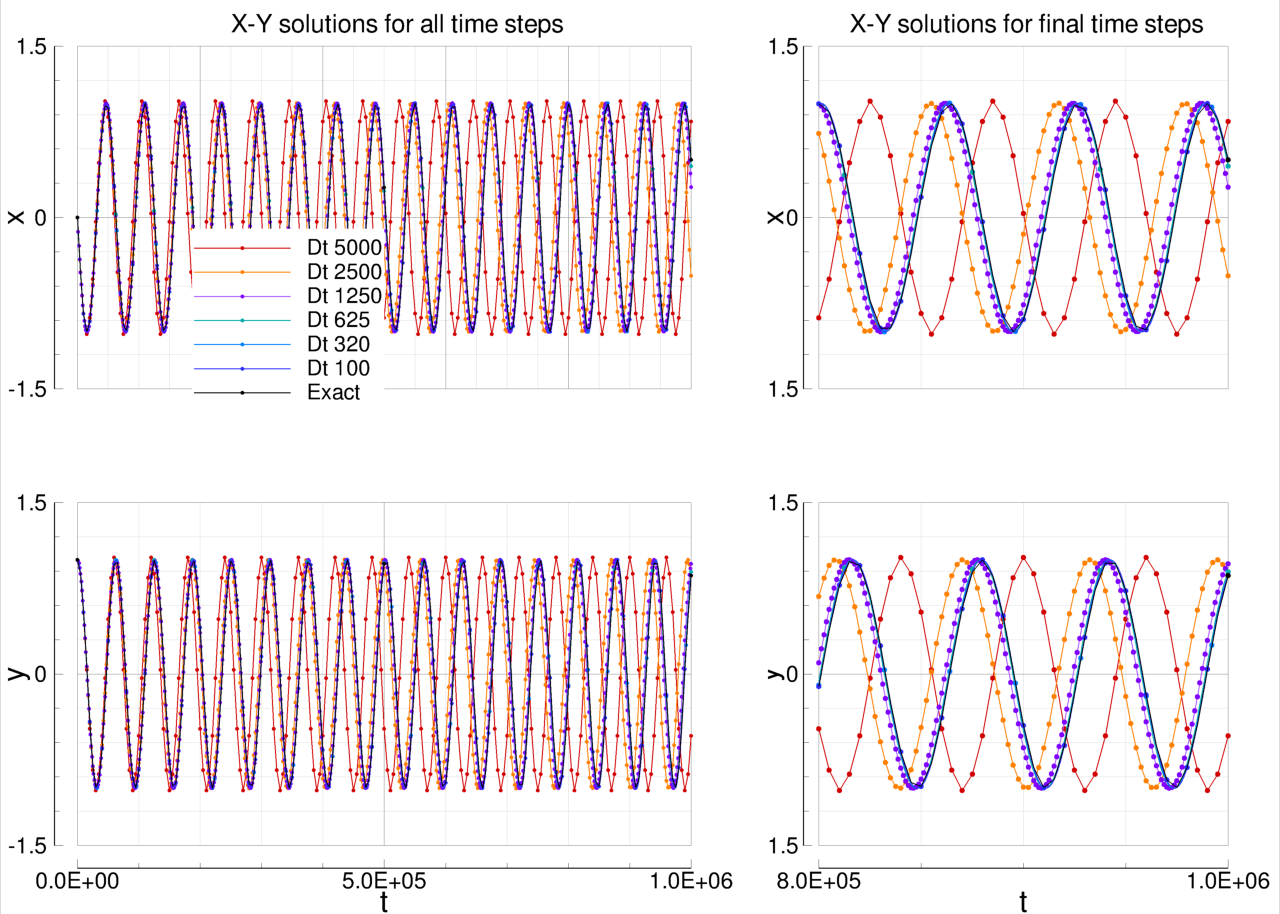
\includegraphics[width=0.70\textwidth]{errors-analysis/oscillation/errors_analysis-oscillation-leapfrog.png}
  \caption{Oscillation equations solutions computed by means of leapfrog 2 steps solver}\label{fig:results-oscillation-leapfrog}
\end{figure}

\paragraph{Low Storage Runge-Kutta}

\begin{figure}[!ht]
  \centering
  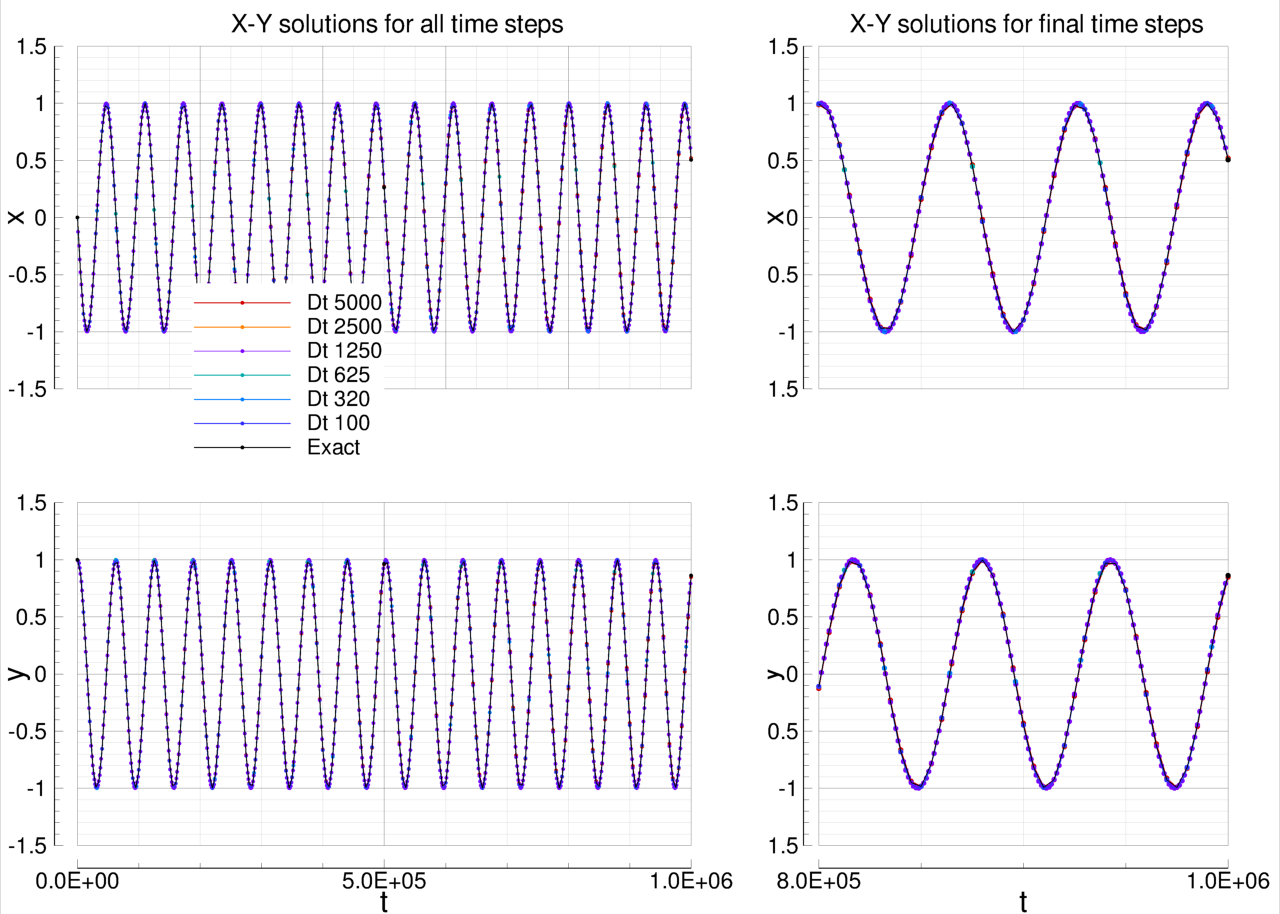
\includegraphics[width=0.70\textwidth]{errors-analysis/oscillation/errors_analysis-oscillation-ls-runge-kutta-5.png}
  \caption{Oscillation equations solutions computed by means of low storage Runge-Kutta 5 stages solver}\label{fig:results-oscillation-ls-runge-kutta-5}
\end{figure}

\paragraph{TVD/SSP Runge-Kutta}

\begin{figure}[!ht]
  \centering
  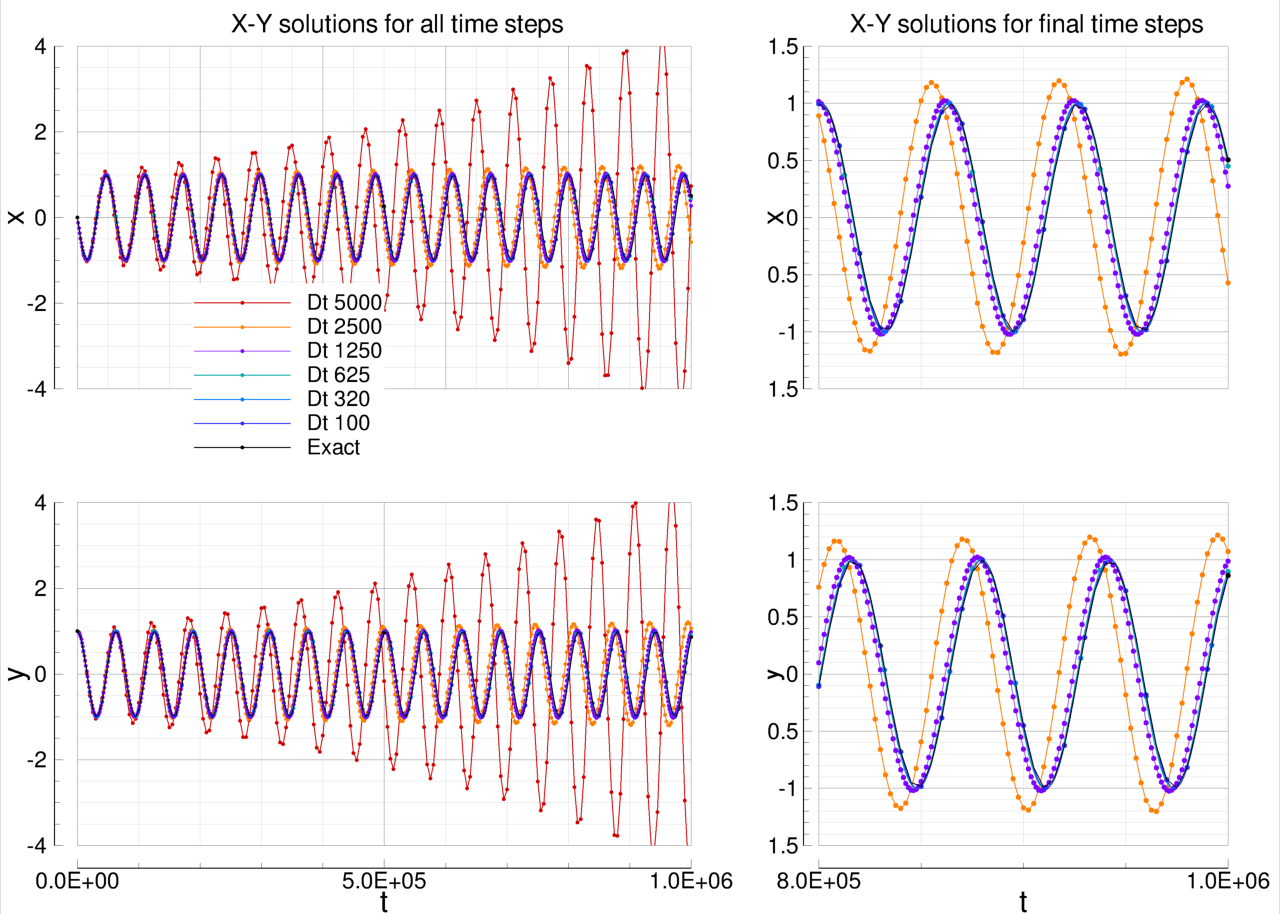
\includegraphics[width=0.70\textwidth]{errors-analysis/oscillation/errors_analysis-oscillation-tvd-runge-kutta-2.png}
  \caption{Oscillation equations solutions computed by means of TVD/SSP Runge-Kutta 2 stages solver}\label{fig:results-oscillation-tvd-runge-kutta-2}
\end{figure}

\begin{figure}[!ht]
  \centering
  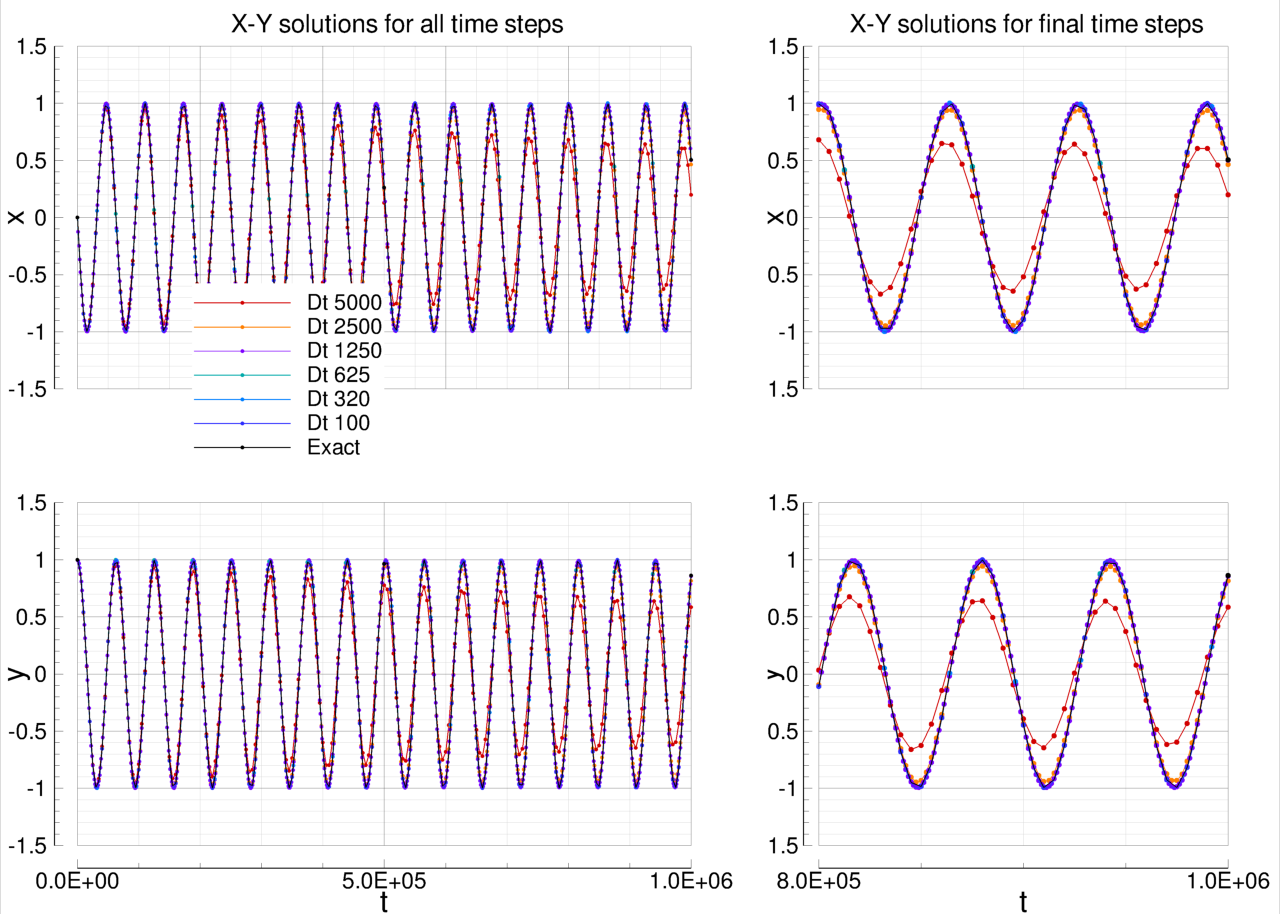
\includegraphics[width=0.70\textwidth]{errors-analysis/oscillation/errors_analysis-oscillation-tvd-runge-kutta-3.png}
  \caption{Oscillation equations solutions computed by means of TVD/SSP Runge-Kutta 3 stages solver}\label{fig:results-oscillation-tvd-runge-kutta-3}
\end{figure}

\begin{figure}[!ht]
  \centering
  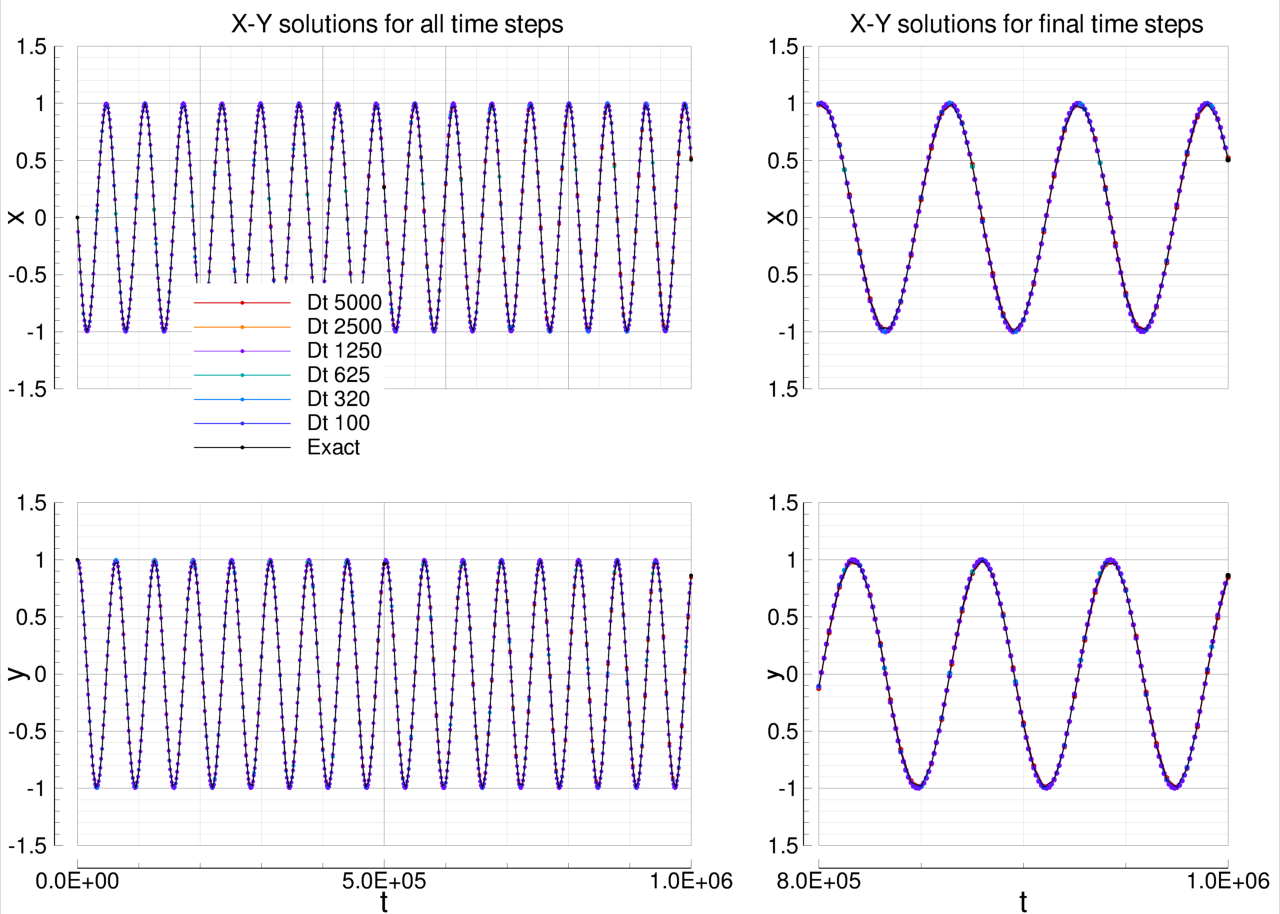
\includegraphics[width=0.70\textwidth]{errors-analysis/oscillation/errors_analysis-oscillation-tvd-runge-kutta-5.png}
  \caption{Oscillation equations solutions computed by means of TVD/SSP Runge-Kutta 5 stages solver}\label{fig:results-oscillation-tvd-runge-kutta-5}
\end{figure}

\clearpage

\section{Ongoing Development Activities}\label{sec:ongoing}

{\color{red} To be written.}

\section{Concluding Remarks and Perspectives}\label{sec:conclusions}

{\color{red} To be written.}

\bibliographystyle{mycpc2}
\bibliography{Reference}

\end{document}
